\documentclass[conference,12pt]{IEEEtran}

\usepackage[tight,footnotesize]{subfigure}

\ifCLASSINFOpdf
  \usepackage[pdftex]{graphicx}
  \graphicspath{{./images/}}
\else
\fi

\usepackage[cmex10]{amsmath}


\hyphenation{op-tical net-works semi-conduc-tor}

\begin{document}
	
\title{System Design Project
	\\Group 12 - Robot Unicorn Defenders
	\\Group report 3}

\author{
\IEEEauthorblockN{Jonas Galdikas, Calum Jackson, Daria Kuznetsova, 
Roberto Bezoari,\\ Marc Howarth, Juozas Kaziukenas, Biser Hong, 
Aleksandar Krastev, Behzad Tabibian}
\IEEEauthorblockA{University of Edinburgh}
}
	
\maketitle
\numberwithin{equation}{section}
\IEEEpeerreviewmaketitle

\pagebreak
	
\section{Introduction}
At the time of the last milestone, we noticed a number of things that we needed to work on. These included:
\begin{itemize}
\item Improving speed of robot movement.
\item Improving the accuracy of robot movement, especially with regard to turning.
\item Developing more game strategies, especially for defensive playing.
\item Structurally adapting the robot to deal with a real-life match. 
\item Adjusting the touch sensors used for collision detection to maximise efficiency.
\end{itemize}
The first friendly tournament also gave a chance to see how our robot fared in a game situation for the first time. This experience brought to light another significant change that we needed to make: a way to stop the robot running without the need to then reconnect to the server via bluetooth, as this is very time consuming. The first friendly tournament also gave a chance to see how our robot fared in a game situation for the first time. \\This experience brought to light another significant change that we needed to make: a way to stop the robot running without the need to then reconnect to the server via bluetooth, as this is very time consuming. 

\section{Organisation}
In this period of the System Design Project, we organised tasks by means of to-do lists and tables on our group website. This divided the work into small, manageable tasks which could then be assigned to specific individuals. The individual in question was then expected to amend the task list upon completion, marking their assignments as done along with any additional useful information. Individual logs were also expected on the website, to report any work they done, so that everyone in the group would be able to tell at a glance what had been accomplished by anyone else.   

\section{Robot Construction}	
During testing and the friendly matches it was apparent the plate holder was impeding access to the NXT brick, wasting game time when the robots were being reset as the holder had to be taken off and replaced. Instant access to the NXT brick was gained by putting the plate holder on a hinge, allowing the plate to be flipped upwards. Additionally, the plate holder was moved further back, to prevent the plate covering the ball at the front of the robot, and attached more securely to prevent it becoming dislodged during the match. \\
We considered building a protective frame around the body of the robot, as many of the teams have been using. However, it quickly became apparent the frame interfered with two things, namely access to the NXT brick ports and also our initial design philosophy, which was to build a small, lightweight robot that would move very fast. Instead, the robot was structurally reinforced by adding more lego connections between the chassis, NXT brick, and kicker, better protecting the integrity of the robot during heavy collisions. The result is a very structurally sound, yet lightweight, construction. Finally, the previously bulky kicker was reconstructed to be lighter, enabling a faster kick, and moving the kicker further back on the robot so that no part of it protruded further forward than the touch sensors used for collision detection, an issue which had given us some trouble during testing. The new arrangement ensured that upon collision the touch sensors are the first part of the robot to experience pressure, allowing the collision to be optimally detected (that is, for the sensors to be fully depressed) and dealt with.

\section{Strategy}
Since the last milestone, a lot of time has been spent making our code more readable and tweaking thresholds in preparation for the first tournament. Integration has been key, as we  began merging all the strategies together including the Potential Fields algorithm. 
We greatly improved our strategy in the following ways:
\begin{itemize}
\item Integrating the Potential Field planning algorithm into low level robot movement. This made robot movement much faster, however, since it is a reactive algorithm, it is vulnerable to possible noises in Vision stack.
\item Creating methods to overcome situations such as if a destination point was outside of the pitch, if the opponent has possession of the ball, or if the touch sensors were activated.
\item Creating an alternative attacking strategy for when the ball is close to the wall, which will try and kick the ball against the wall at such an angle that the ball will head towards the  opponent goal, Figure \ref{fig:bounceWall}.
\begin{figure}[htp]
\begin{center}
\leavevmode
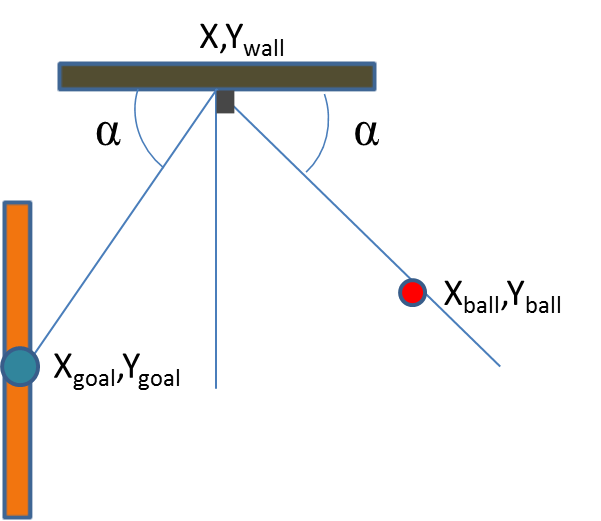
\includegraphics[width=0.2\textwidth] {getBallWall.png}
\end{center}
\caption{Position of Different objects near wall. Aim is to calculate $X$ given other positions}
\label{fig:bounceWall}
\end{figure}
\item Altering the methods calculating the obstacle avoidance point to implement a dynamic point instead of a static point.
\item Writing a strategy for predicting the position of a moving ball, using a circular buffer data structure, which stores the previous positions of the ball from vision updates.
\item Integrating strategy classes together into a MainStrategy class, which uses a state system to decide what strategy needs to be called to deal with the current on-pitch situation.
\item Some functions were moved to higher levels to increase their availability to all of the strategies, often specific functions were made more general to increase their usefulness, which led to the removal of many similar/duplicate functions.
\end{itemize}
While playing in the friendly matches we also realised we needed a way to stop the robot running, for example when repositioning it once a goal was scored, without having to then go through the time consuming process of reconnecting to the server via Bluetooth. In light of this, we extended the GUI for our program to have two buttons: Start/Stop and Start/Stop execution. The former was the similar to the previous Start button, the only difference being that now it doesn't run the strategy once the Bluetooth connection and vision are set up it will wait for Start execution to be clicked. This allows us to not only start moving immediately when we want to, but also lets us change strategy (from main to take-penalty for example) without re-establishing Bluetooth connection.
Related to this, Juozas modified the program running on the robot itself to never quit the program once it's started, which made it easier to test our code on the robot without needing to relaunch the client every time we click Stop on the program.

The Major barrier in using Potential Field algorithm was how we apply the resultant velocity on the robot. This is a challenge since PF algorithm itself does not take into account robot constraints which in turn makes the control problem specific to a nonholonomic robot\cite{book:holonomicity}. Our proposed method transforms calculated vector to $V_{linear}$ and $V_{angular}$ velocities for such a differential drive robot, Figure \ref{fig:robot}.
\begin{figure}[htp]
\begin{center}
\leavevmode
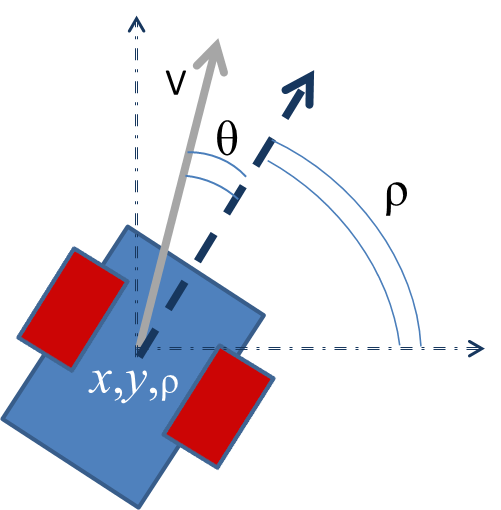
\includegraphics[width=0.2\textwidth] {robot.png}
\end{center}
\caption{Simple model of nonholonomic differential drive robot}
\label{fig:robot}
\end{figure}
Following equations demonstrates how we apply the velocity vector to the robot:
\begin{align}
\label{equ:PFVelocity}
V_{linear} = \begin{Vmatrix}v\end{Vmatrix} cos(\theta) ,
V_{angular} = {1 \over \begin{Vmatrix}v\end{Vmatrix}} \theta
\end{align}
The proposed method has prevents robot from making sharp turns while it is not close to the destination point and therefore starts to make sharper turns as it gets closer to destination. Also, angular velocities are controlled with a minimum and maximum velocities so robot never tries to turn faster than some specific threshold.
\section{Vision}
Since last milestone most of the work on the Vision stack was focused on cleaning up the code and documenting what has been done. A complete documentation of API and different functionalities of the robot is created using DoxyGen\cite{web:DoxyGen} tool.
The code base was split into three sub-modules:
\begin{itemize}
\item Utilities: helper functions to load parameters from input, loading images etc.
\item Machine Learning: A complete set of functions used to train and predict different objects from the image using SVM(Support Vector Machines).
\item Main: Main functionalities including contour detection, image preprocessing (i.e image subtraction and color space transformations).
The goal was to make this code available for public use.
\end{itemize}
 
\section{Simulator}
The major improvements to the simulator were restructuring of the code base, implementing a generalized collision detection algorithm, and providing the strategy module with additional drawing capabilities.
Having had troubles managing all collisions by passing objects around to all other objects, a central collision detection mechanism was designed. Objects that need support for collisions are registered with a collision detector and all relevant parties are notified in the case of collision. The collision detector requests each object to send their shape on every update cycle. For every corner of that shape a test is made to establish whether it falls within any of the other registered objects' shape. If this is the case, a collision packet, which includes the type of collision and the side of the shape that is closest to the other shape's corner, is constructed and sent to each object participating in the collision. 
As the strategy was becoming more and more complex, efficient debugging methods needed to be employed, especially in the case of finding logical errors in the code, which were usually harder to detect. Since any strategy involves fine tuning and certain thresholds are inevitable, a simple but useful transparent oval is drawn whenever there was a need to visualize, for example, the area around a point to which the robot needs to move. This ensures calculations were always correct and the strategy was proceeding as it should.


\section{Conclusion}
The improvements that we decided on at the start of this phase were successfully implemented, and any new problems were dealt with with a good degree of efficiency. Our progress to the semi-final stage of the first friendly tournament, and thus a seeded position for the second tournament, is encouraging. We hope to continue the good work up until the final stages of the System Design Project, and improve on our semi-final result in the upcoming games.

\bibliographystyle{IEEEtran}
\bibliography{bibliography}
\end{document}
